\section{Results}\label{sec:Results}

\subsection{Regression on generated data}
The performance of the ordinary least squares fit to the data is shown for different model complexities in figure \ref{fig:ols_frankie_train_test_bias_variance} (left). The prediction on test data has a minimum mean squared error of $\text{MSE} = 0.0136$ and $R^2 = 0.819$ (not shown in the plot), which occurs when the model complexity is of degree $d=5$, while the prediction on the training data has no minimum and keeps declining for higher complexity. The plot to the right in the same figure shows again the mean squared error of the predictions on the test data, and also its decomposition into bias$^2$ and variance. 
\begin{figure}[!h]
    \centering
    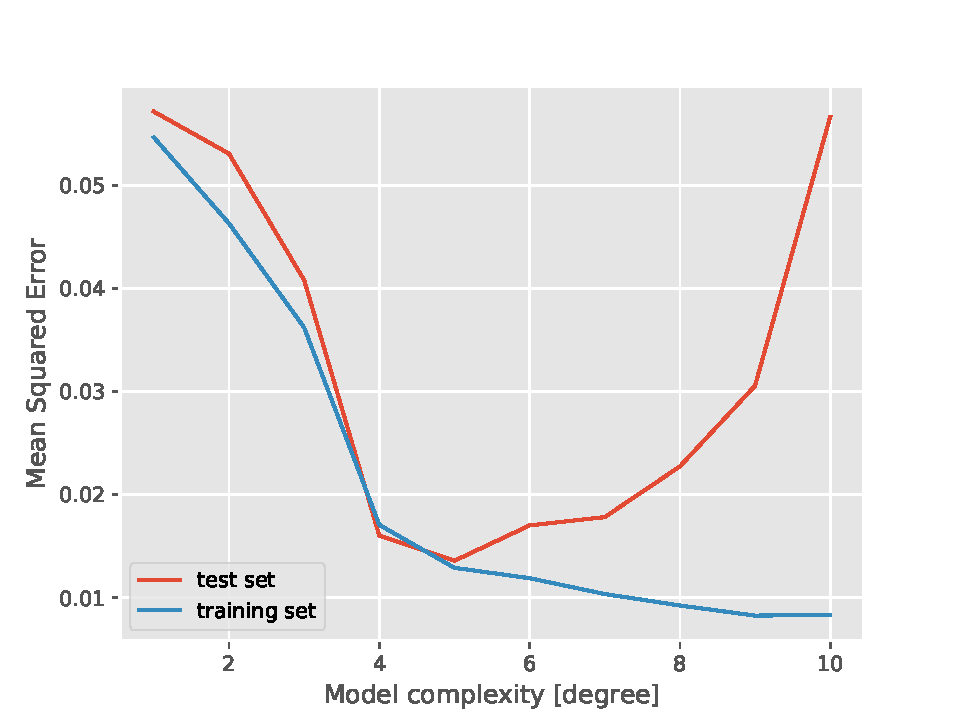
\includegraphics[scale=0.48]{Figures/OLS/deg_analysis_ols_test_train_001.pdf}
    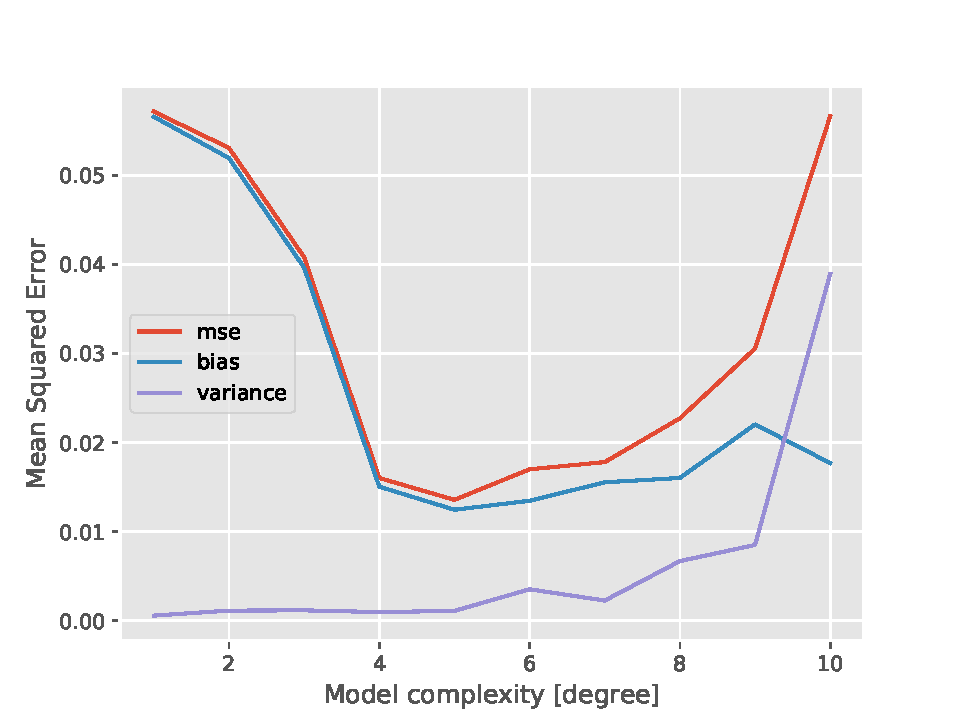
\includegraphics[scale=0.48]{Figures/OLS/deg_analysis_ols_bias_variance_002.pdf}
    \caption{Error in the OLS regression prediction on the generated data as a function of the models polynomial degree for the training and testing data (left). Figure to the right shows the bias$^2$ and variance decomposition of the MSE in the prediction on the test data.}
    \label{fig:ols_frankie_train_test_bias_variance}
\end{figure}
Figure \ref{fig:ols_frankie_confidence} also shows the confidence intervals of the different $\beta$ parameters for the optimal model with $d=5$.

For Ridge regression, figure \ref{fig:ridge_heatmap_frankie} shows the mean squared errors in the predictions on the test data for values of the hyper parameter $\lambda$ and polynomial degree $d$. The minimum error is at $\lambda = 10^{-4}$ and $d = 9$, with $\text{MSE} = 0.0139$\footnote{In the plot we see that the MSE is truncated at $0.013$, but an inspection of the data showed that the actual value was $0.0139$.} and $R^2 = 0.874$.
\begin{figure}[!h]
    \centering
    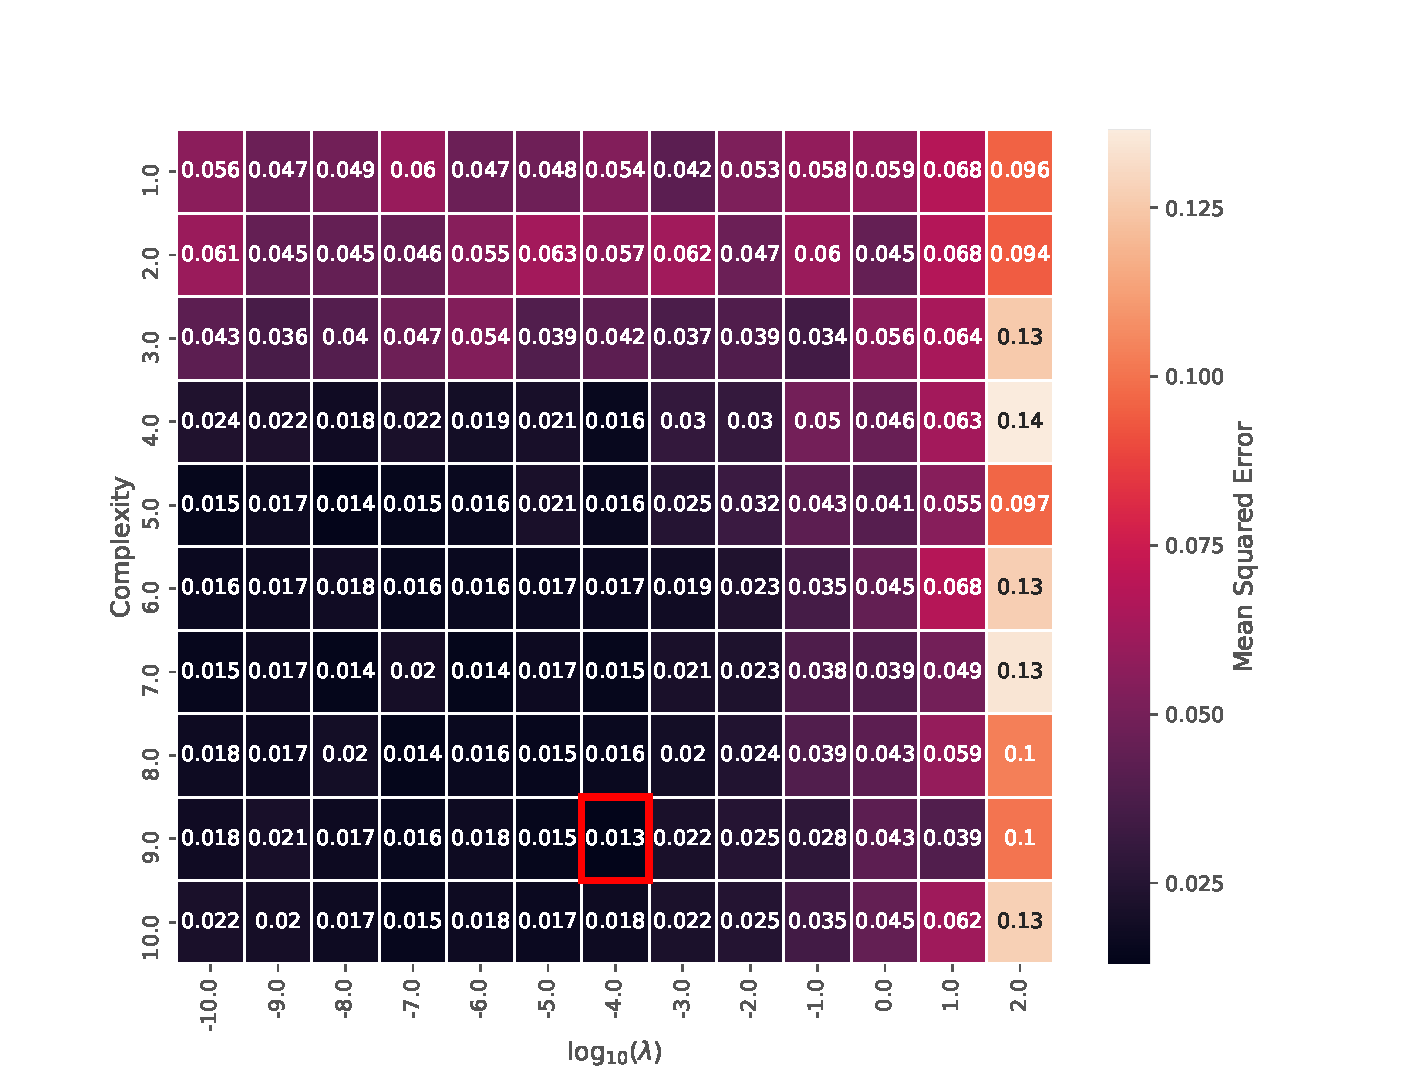
\includegraphics[scale=0.6]{Figures/RIDGE/min_mse_heatmap_ridge_003.pdf}
    \caption{Heat map of the MSE of the predictions of Ridge regression on the generated data for different values of $\lambda$ and model complexity $d$.}
    \label{fig:ridge_heatmap_frankie}
\end{figure}
\begin{figure}[!h]
    \centering
    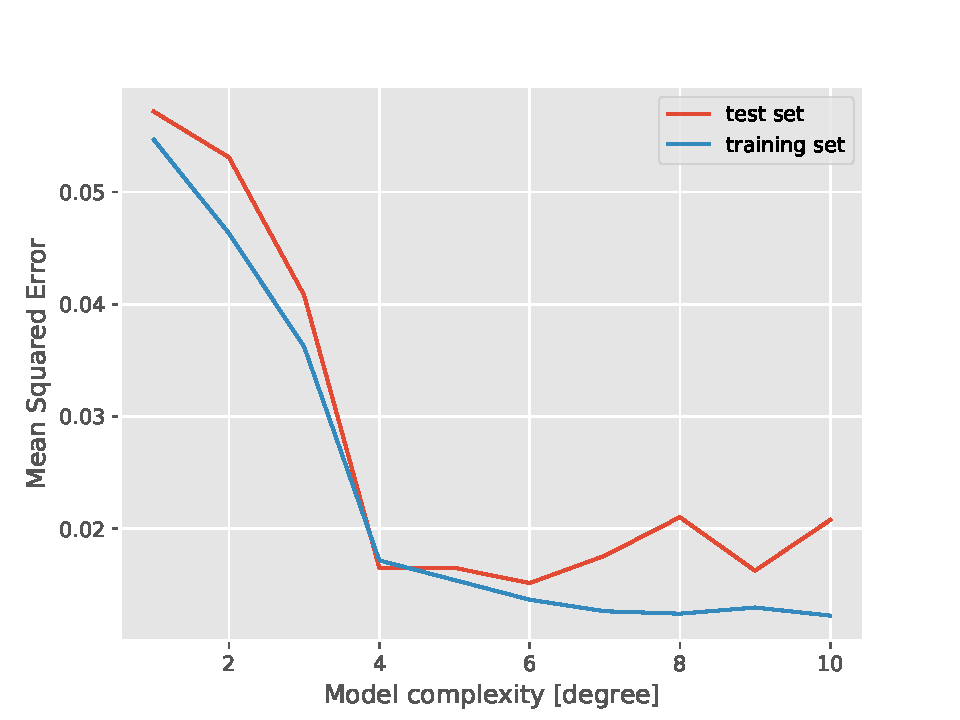
\includegraphics[scale=0.48]{Figures/RIDGE/deg_analysis_ridge_test_train_004.pdf}
    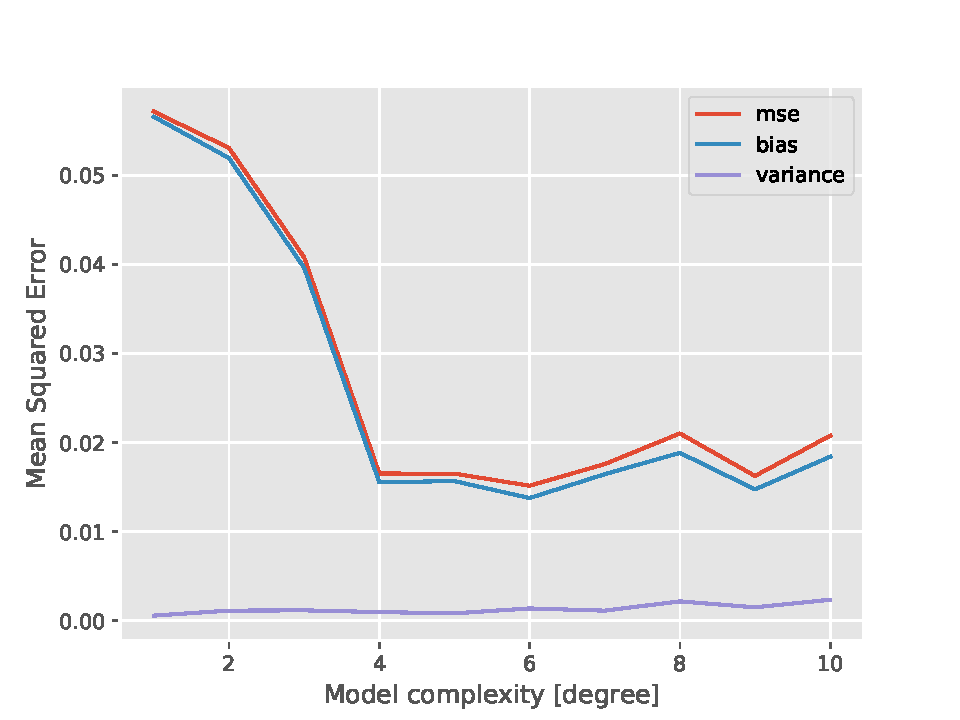
\includegraphics[scale=0.48]{Figures/RIDGE/deg_analysis_ridge_bias_variance_005.pdf}
    \caption{Error in the Ridge regression prediction on the generated data as a function of complexity, with $\lambda = 10^{-4}$. The left plot shows the error in the prediction on both the training and test data. The right plot shows the bias$^2$ and variance decomposition of the MSE on the test data.}
    \label{fig:ridge_frankie_train_test_bias_variance}
\end{figure}
Figure \ref{fig:ridge_frankie_train_test_bias_variance} shows the performance of Ridge regression in a separate run for different polynomial orders $d$, with the optimal value of $\lambda = 10^{-4}$ found in the above figure (\ref{fig:ridge_heatmap_frankie}). The figure shows the errors in both predictions on the test data and training data, as well as the bias$^2$ and variance decomposition of the error. Here we found the minimum predicted MSE to occur at $d = 6$, with $\text{MSE} = 0.151$ and $R^2 = 0.877$.


\begin{figure}[!h]
    \centering
    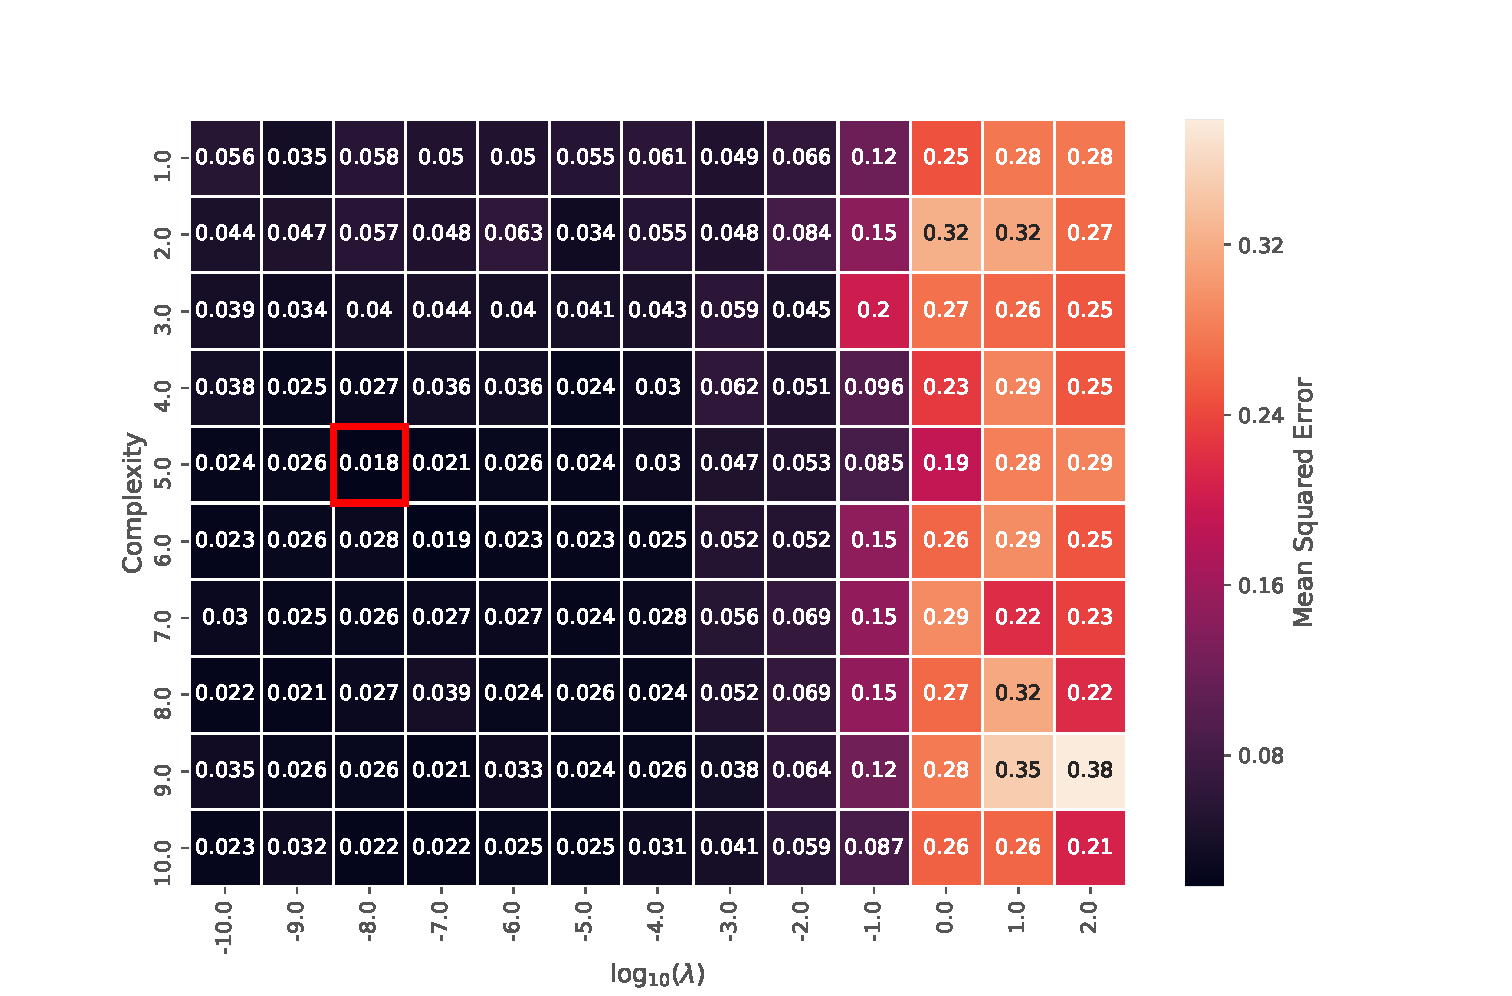
\includegraphics[scale=0.6]{Figures/LASSO/min_mse_heatmap_ridge_019.pdf}
    \caption{Heat map of the MSE of the predictions of Lasso regression on the generated data for different values of $\lambda$ and model complexity $d$. Tolerance for convergence of the gradient descent: 0.0001, maximum iterations: 10000.}
    \label{fig:lasso_heatmap}
\end{figure}

Figure \ref{fig:lasso_heatmap} shows the analysis of Lasso regression applied to the Franke function, with respect to the model complexity and the hyper parameter $\lambda$. The minimum mean squared error, $\text{MSE} = 0.0183$ was found with a polynomial degree of $d=5$ and $\lambda = 10^{-8}$, and had a corresponding $R^2$-score of $0.7874$.



\begin{figure}[!h]
    \centering
    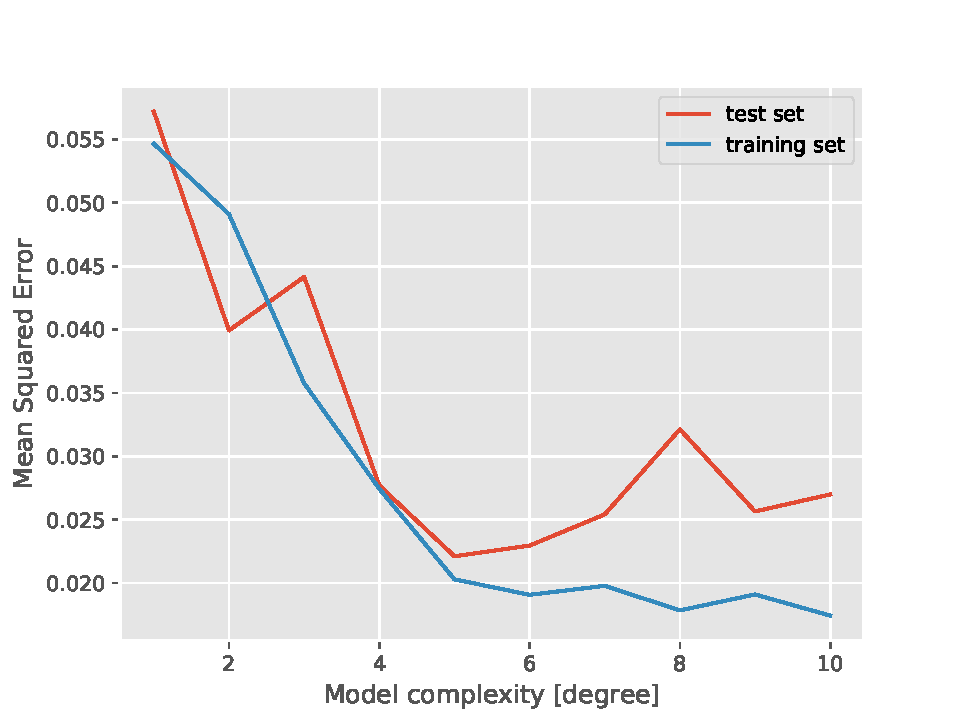
\includegraphics[scale=0.48]{Figures/LASSO/deg_analysis_lasso_test_train_020.pdf}
    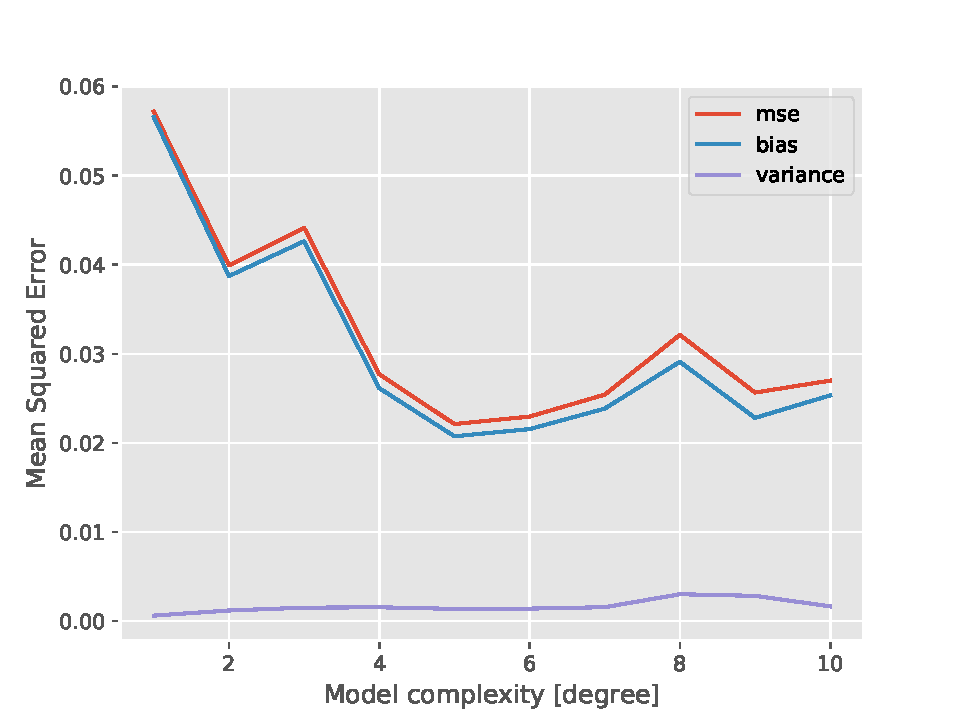
\includegraphics[scale=0.48]{Figures/LASSO/deg_analysis_lasso_bias_variance_021.pdf}
    \caption{Error in the Lasso regression prediction as a function of complexity, with $\lambda = 10^{-8}$, when modeling on the Franke data set. The left plot shows the error in the prediction on both the training and test data. The right plot shows the bias$^2$ and variance decomposition of the MSE on the test data. Tolerance for convergence of the gradient descent: 0.0001, maximum iterations: 10000.}
    \label{fig:lasso_test_train_bias_variance}
\end{figure}

In figure \ref{fig:lasso_test_train_bias_variance} we see the Lasso regression performed for different polynomial degrees, for the optimal value $\lambda=10^{-8}$. The plots shows the MSE for the training and test set, and how the MSE, bias$^2$ and variance behaves as a function of model complexity.


\begin{table}[!h]
    \caption{Comparison of the models with the lowest MSE for each regression method, applied to the Franke function data set.}
    \label{tab:franke}
    \begin{tabular}{|l|c|c|l|l|}
        \hline
        Method & degree & $\text{log}_{10} \lambda$ & MSE     & $R^2$  \\ \hline
        OLS    & 5 &  & 0.0136  & 0.819  \\ \hline
        Ridge  & 6 & -4 & 0.0139  & 0.877  \\ \hline
        Lasso  & 5 & -8 & 0.0183 & 0.728 \\ \hline
    \end{tabular}
\end{table}


\begin{figure}[!h]
    \centering
    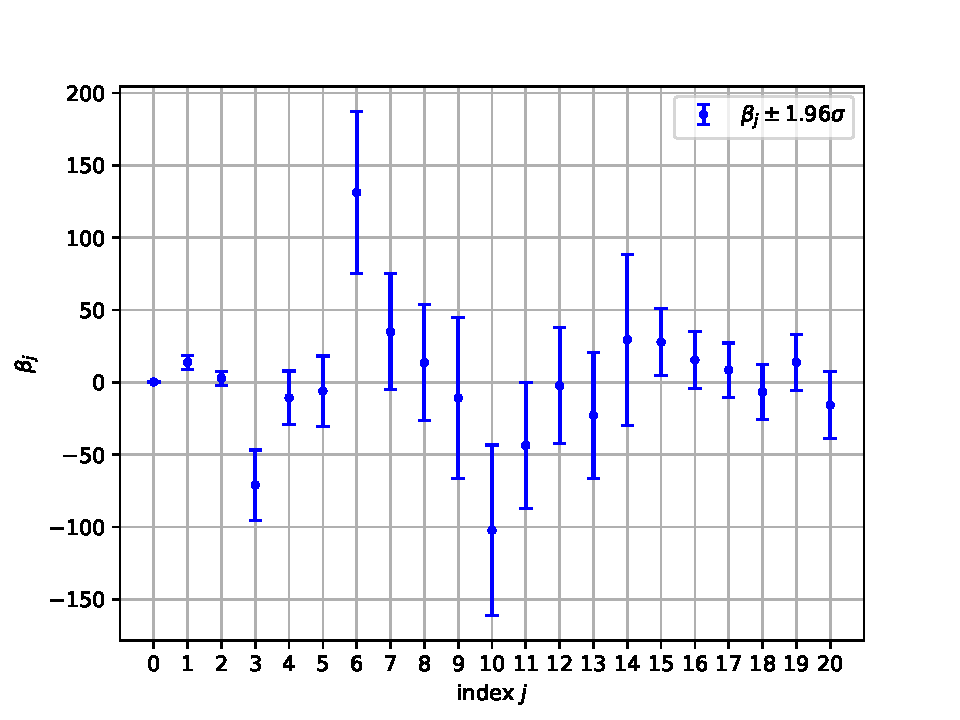
\includegraphics[scale=0.48]{Figures/OLS/confidence_interval_betas_024.pdf}
    \caption{The parameters $\beta_j$ for OLS with a confidence interval of $95\%$. Lower indices correspond to lower polynomial term coefficients, and vice verca.}
    \label{fig:ols_frankie_confidence}
\end{figure}


\subsection{Regression on real terrain data}

By doing an analysis of model complexities $d \in [1, 10]$ and hyper parameters $\log_{10}(\lambda) \in [-10, 2]$ with $100$ bootstraps, we have in table \ref{tab:terrain} listed the predicted errors of the best model configuration of the three regression methods on the real data (see section \ref{sec:data_format}). All three methods favor a polynomial of degree $d=10$, with OLS having the smallest estimate of the error, $\text{MSE} = 0.0091$. The Ridge and Lasso methods yield the best results with small values of the hyper parameter, $\lambda_{Ridge} = 10^{-9}$ and $\lambda_{Lasso} = 10^{-10}$ respectively. Figure \ref{fig:bias_variance_all_methods} shows the bias-variance decomposition of the estimated errors for the three methods for different polynomial degrees. The curve representing the MSE (the red curve) lies directly underneath the curve of the bias$^2$, and is therefore not visible in the three plots. The confidence intervals of the OLS $\beta$ parameters are shown in  \ref{fig:OLS_terrain_confidence_intervals}. In figure \ref{fig:model_terrain} we have plotted the data along side the predicted values of the OLS model with the optimal parameters found in table \ref{tab:terrain}. The appendix (sec. \ref{sec:Appendix}) contains additional plots of the results of the tuning of the $\lambda$ and $d$ parameters on the terrain data for Ridge and Lasso, as well as the error in the predictions on the test and training data for all of the three methods.

\begin{table}[!h]
    \caption{Comparison of the models with the lowest MSE for each regression method, applied to the terrain data set.}
    \label{tab:terrain}
    \begin{tabular}{|l|c|c|l|l|}
        \hline
        Method & degree & $\text{log}_{10}(\lambda)$ & MSE     & $R^2$  \\ \hline
        OLS    & 10 & - & 0.0091  & 0.6323  \\ \hline
        Ridge  & 10 & -10 & 0.0092  & 0.6325  \\ \hline
        Lasso  & 10 & -9 & 0.0138 & 0.0157 \\ \hline
    \end{tabular}
\end{table}


\begin{figure}[!h]
    \centering
    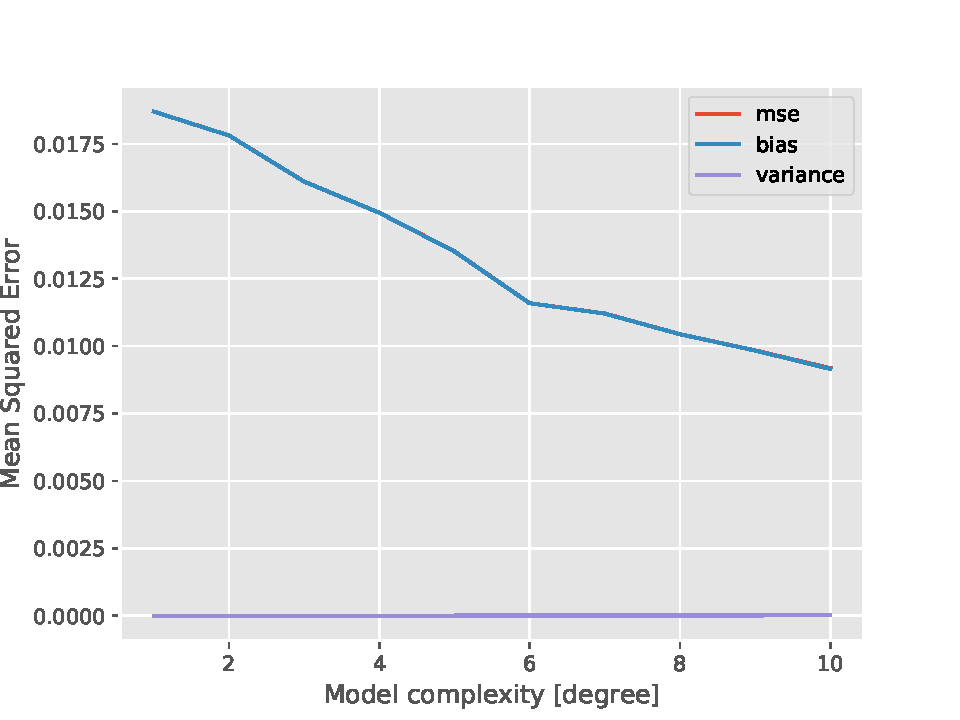
\includegraphics[scale=0.48]{Figures/RealDataPlots/deg_analysis_ols_bias_variance_016.pdf}
    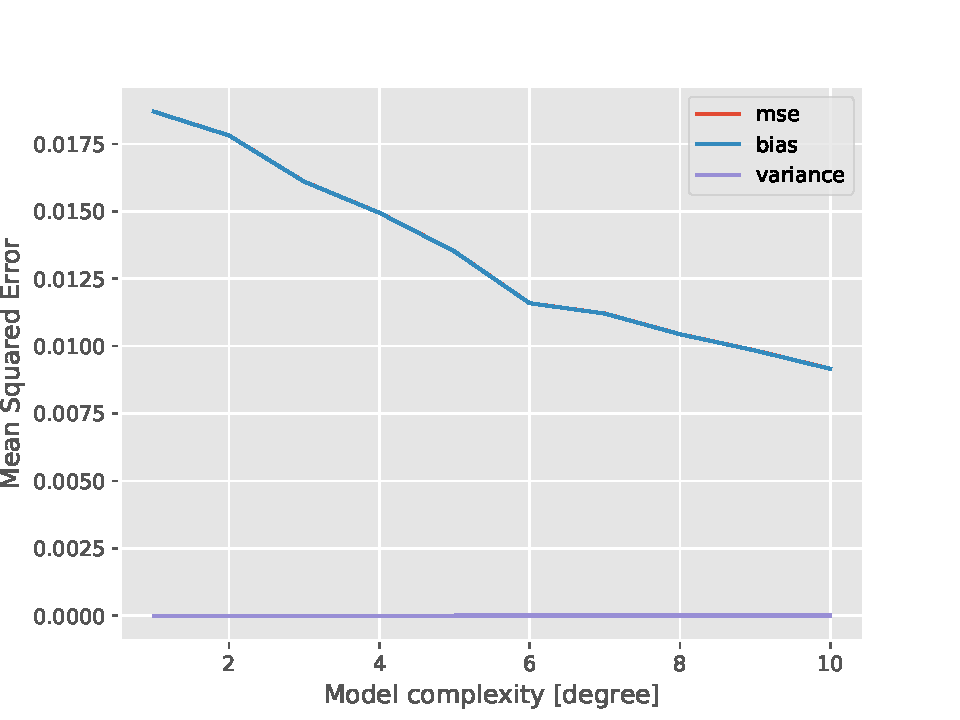
\includegraphics[scale=0.48]{Figures/RealDataPlots/deg_analysis_ridge_bias_variance_012.pdf}
    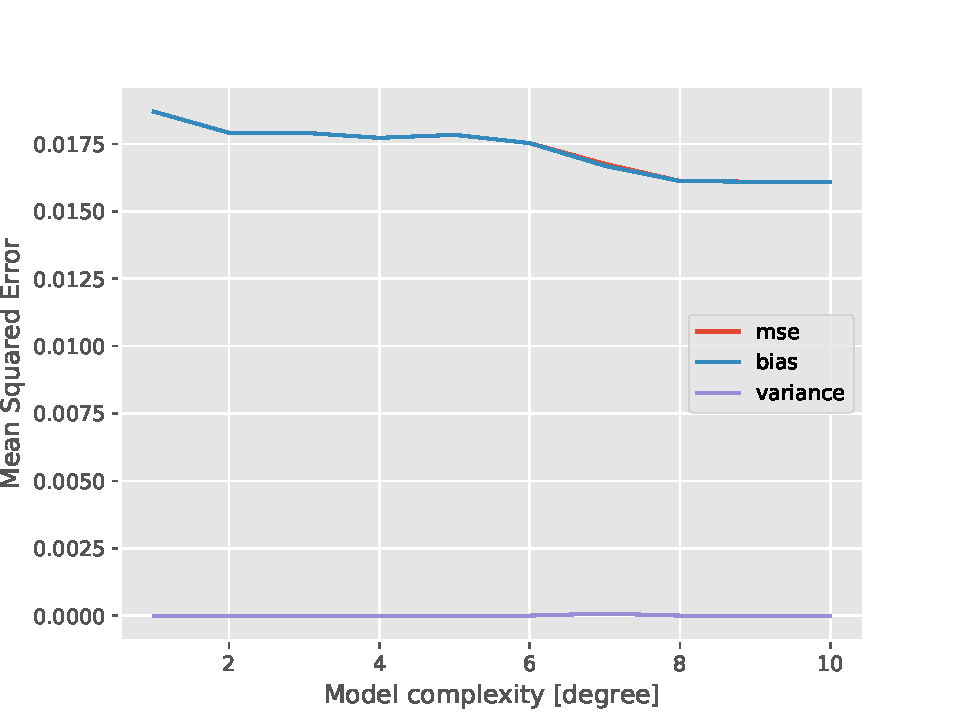
\includegraphics[scale=0.48]{Figures/RealDataPlots/deg_analysis_lasso_bias_variance_026.pdf}
    \caption{Estimated prediction errors of OLS (top left), Ridge (top right) and Lasso (bottom), and their bias$^2$ - variance decomposition as a function of model complexity.}
    \label{fig:bias_variance_all_methods}
\end{figure}

\begin{figure}[!h]
    \centering
    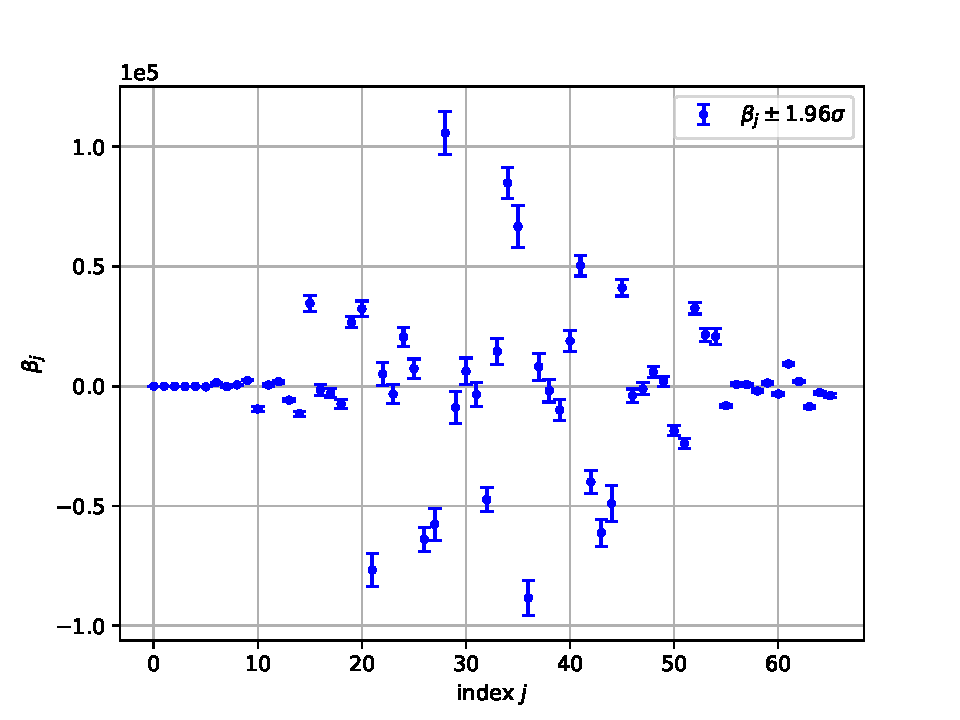
\includegraphics[scale=0.48]{Figures/RealDataPlots/confidence_interval_betas_028.pdf}
    \caption{The parameters $\beta_j$ for OLS with a confidence interval of 95\%. Lower indices correspond to lower polynomial term coefficients, and vice verca.}
    \label{fig:OLS_terrain_confidence_intervals}
\end{figure}


\begin{figure}[!h]
    \centering
    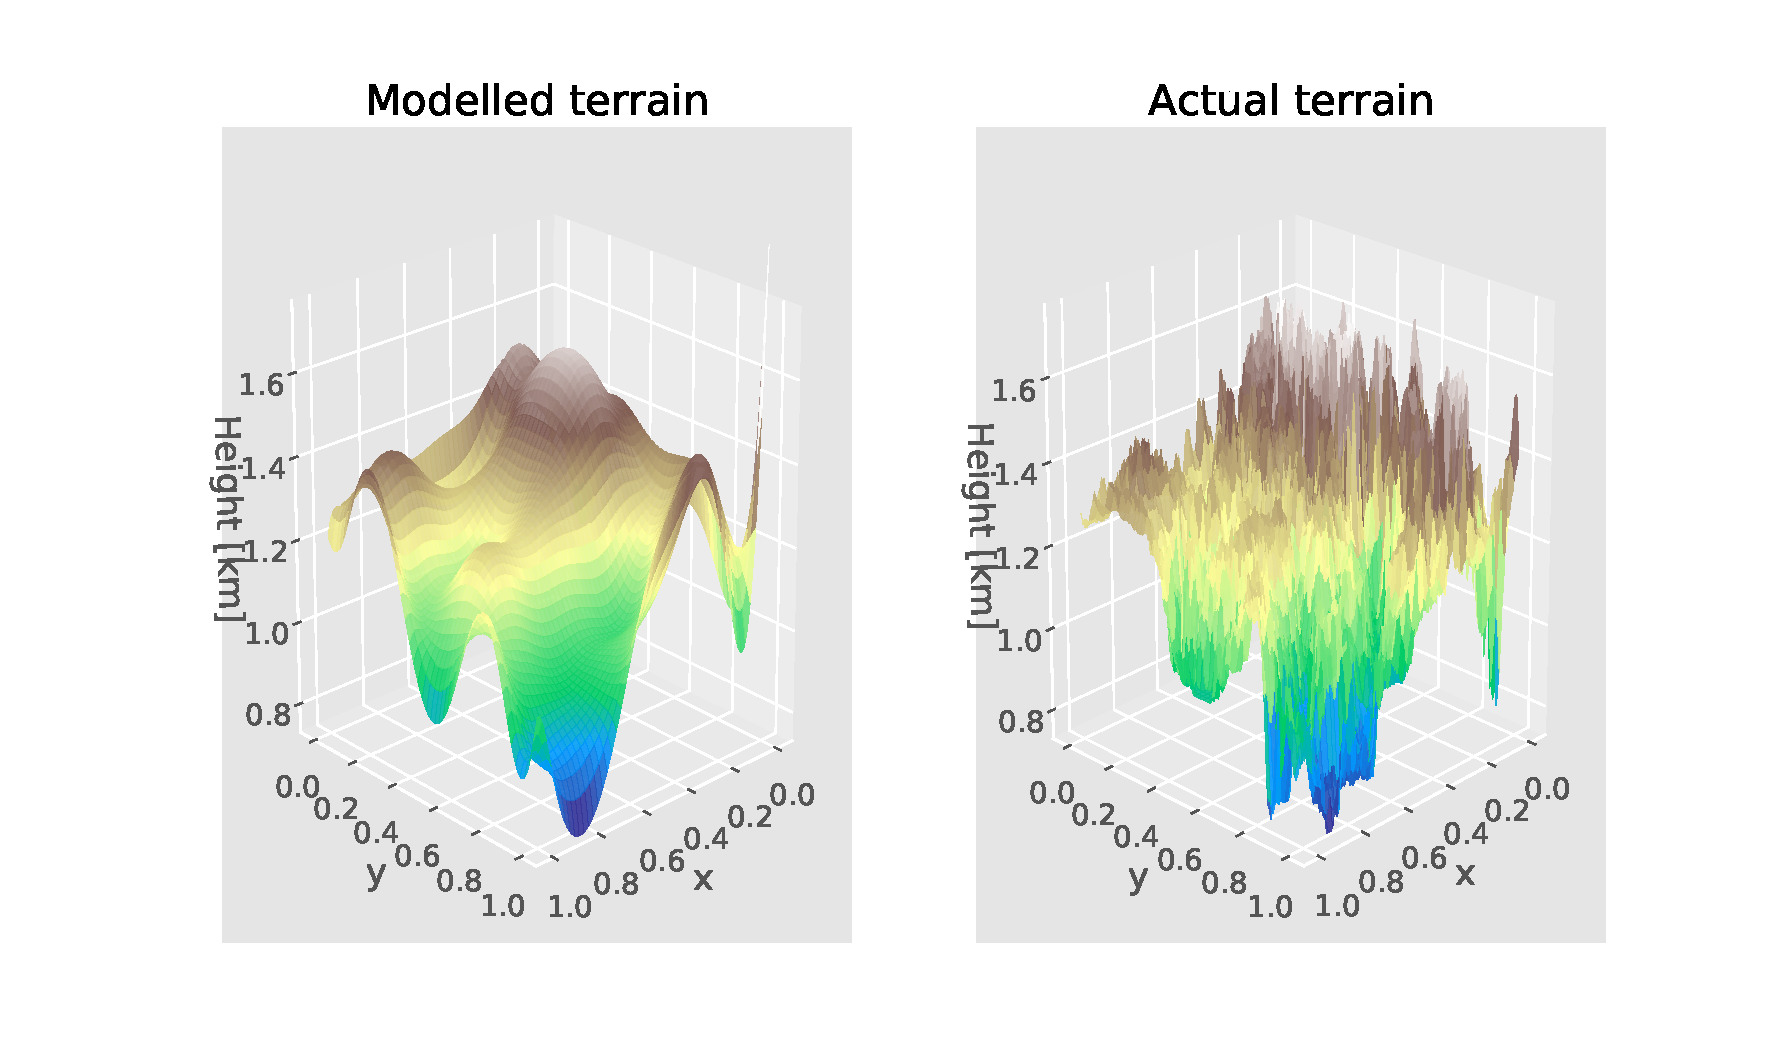
\includegraphics[scale=0.6]{Figures/RealDataPlots/model_vs_terrain_023.pdf}
    \caption{Height maps of the modelled terrain (left) and the terrain data(right).}
    \label{fig:model_terrain}
\end{figure}